\section{Imaging}

% http://en.wikipedia.org/wiki/Free_induction_decay
% In Fourier Transform NMR, a free induction decay (FID) is the
% observable NMR signal generated by non-equilibrium nuclear spin
% magnetisation precessing about the magnetic field (conventionally
% along z). 

% B1 magnetic field

To distinguish slices in the body, a gradient field, $B_{G_s}$, is applied
along the z-axis. The gradient field varies along the z-axis, with
only a 0 Tesla effect in the slice that should be excited. Since the
frequency of the photons that can excite a spin is linearly
proportional to the strength of the magnetic field on that spin, it
follows that the photons of frequency $\omega_0 = \gamma B_0$ will
only affect spin packets unaffected by the gradient $B_{G_s}$. Applying
$B_{G_s}$ for the duration of the RF pulse ensures that only spin packets
in the slice is excited and will produce a signal during the signal
acquisition phase.

In our simulation we assume that the correct slice has been selected
and excited, so we only work with a 2 dimensional image and the net
magnetization vectors have been rotated into the transversal
plane. This allows us to focus on the image acquisition phase.


By Faraday's law of induction the signal generated by a single spin
packet is

\begin{displaymath}
  M^*(t, \mathbf{p}) = M_x(t, \mathbf{p}) + i \cdot M_y(t, \mathbf{p})
\end{displaymath}

The complete signal from the excited slice is then

\begin{displaymath}
  M^*(t) = \sum^{(X, Y)}_{(x',y')} (M_x(t, \mathbf{p_{(x',y')}}) + i \cdot M_y(t, \mathbf{p_{(x',y')}}))
\end{displaymath}

which is sampled in intervals of $t$ for the duration $\tau$.

\subsection{Frequency and phase gradients}

% Constant gradient field along the x axis (read-out direction). The
% strength of the gradient field increases along the x-axis and never
% changes over the course of the signal acquisition.

\begin{displaymath}
  v = \gamma (B_0 + x B_{G_f})
\end{displaymath}


% The y-axis is the phase encode direction and is phase encoded with a
% phase gradient. Phase phase face phase.


\begin{figure}
  \centering
  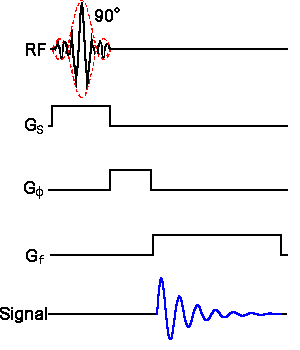
\includegraphics[width=5cm]{gradientSequence}
  \caption{A timing diagram of the application of gradients with
    respect to the RF pulse and signal acquisition.}
  \label{fig:gradientSequence}
\end{figure}



\subsection{K-space}



% Perform 2D fourier transform of the data in k-space, can Sangild's programs do this for us?

\begin{displaymath}
  f(\omega) = \int^\infty_{-\infty}f(t)e^{-i \omega t} dt = \int^\infty_{-\infty}f(t)(\cos(\omega t) - i \sin(\omega t)) dt \approx \sum^\infty_{-\infty}f(t)(\cos(\omega t) - i \sin(\omega t))
\end{displaymath}


%%% Local Variables:
%%% mode: latex
%%% TeX-master: t
%%% TeX-PDF-mode: t
%%% End:
